Die Datenbankverbindung werden grundsätzlich beim Starten des Servers aufgebaut und erst wenn diese erfolgreich waren, wird der Server tatsächlich gestartet. Die Datenbankverbindung in express.js wird grundsätzlich wie folgt aufgebaut:
\newline
\begin{lstlisting}
    const client = new MongoClient(<Connection_String>)
    const result = await client.connect()
    let db = result.db(<Datenbankname>)
\end{lstlisting}
Zuerst wird ein neuer MongoClient erstellt, dabei muss man den Connection-String der Datenbank als Parameter übergeben. Anschließend wird eine Verbindung zur Datenbank aufgebaut, mit dem erhaltenen Objekt kann man sich nun auf alle Collections, die sich in dieser Datenbank befinden, verbinden. Da allerdings im Fall dieser Diplomarbeit zwei unterschiedliche Datenbanken benötigt werden, wurde diese Verbindung auf eine eigene Datei ausgelagert.
\newline
Dazu wurde ein config-File erstellt in welchem die Connection-Strings der beiden Datenbanken als Variablen definiert und als JSON mittels \textbf{module.exports} exportiert werden.
\begin{figure}[h!]
    \centering
    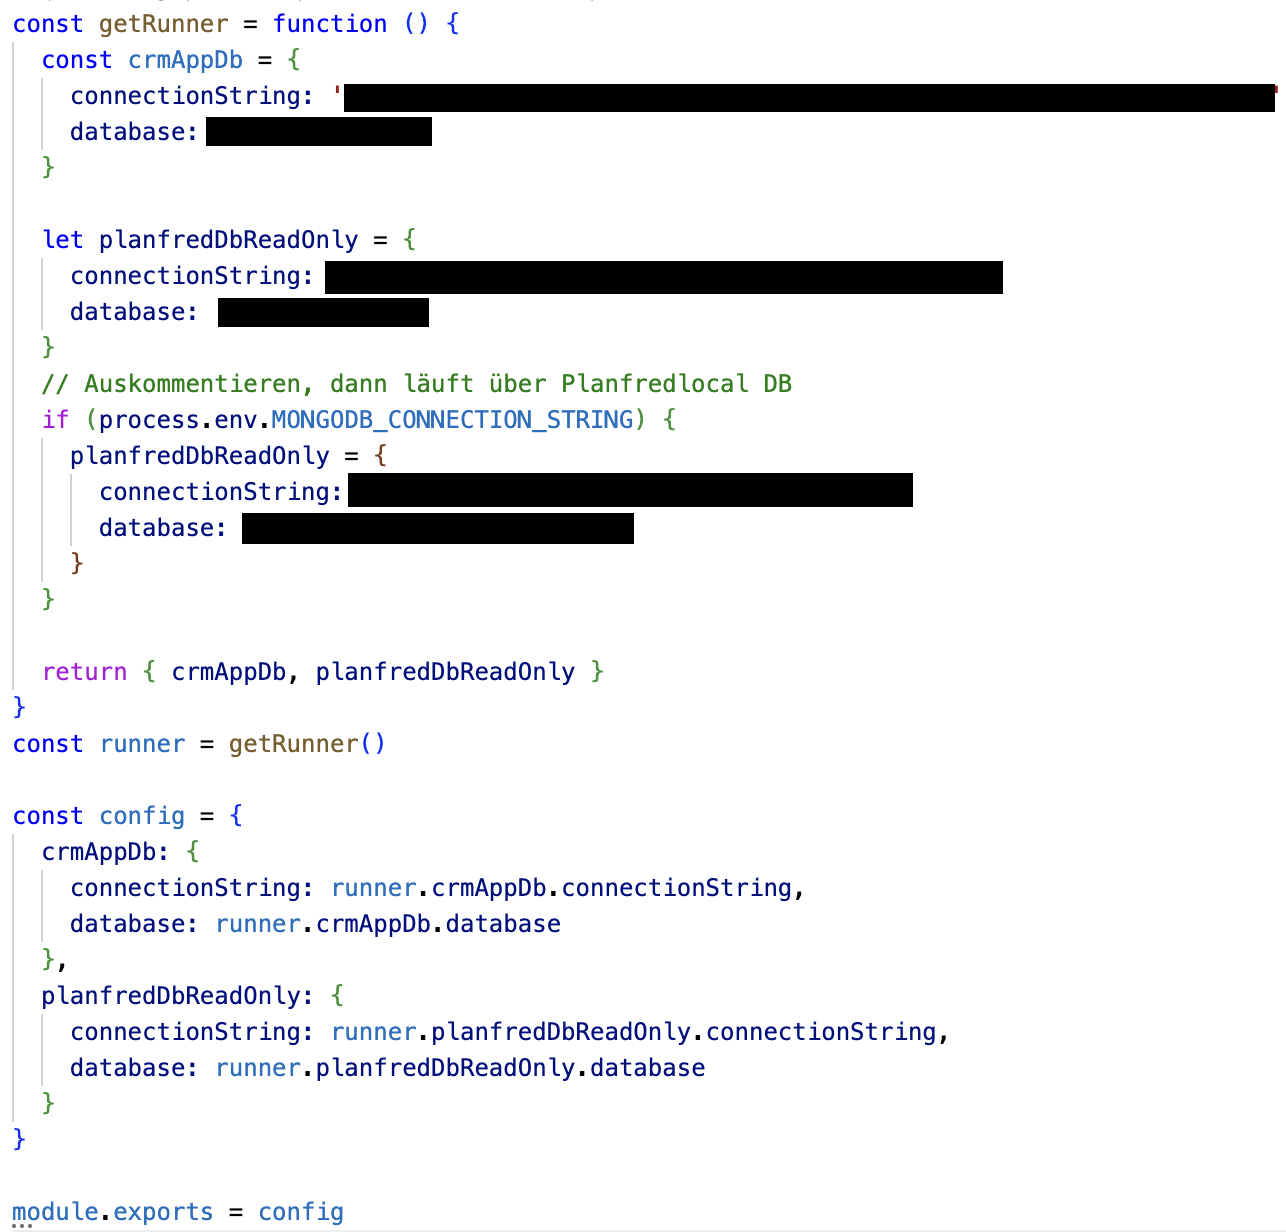
\includegraphics[width=0.5\textwidth]{pics/config-file-conn-strings.png}
    \caption{Config-File}
    \label{fig:enter-label}
\end{figure}
Wie man in dem obigen Screenshot erkennen kann wurde ebenfalls noch die Möglichkeit implementiert durch auskommentieren des if-Statements auf eine Datenbank zuzugreifen, welche weniger Einträge enthält.
\newline
Anschließend wird in einem weiteren File dieses JSON importiert und eine Funktion erstellt in welcher wie im oben gezeigten Beispiel die Verbindung aufgebaut wird.
\begin{lstlisting}
async connect () {
    const client = new MongoClient(this.dbConfig.connectionString)
    const result = await client.connect()
    this.db = result.db(this.dbConfig.database)
    logger.info(`Connected to MongoDB ${this.dbConfig.database}.`)
}
\end{lstlisting}
Diese Funktion wird ebenfalls exportiert und im server.js importiert und aufgerufen. Dabei wird jeweils darauf gewartet, ob der Verbindungsaufbau erfolgreich war, damit es nicht zu dem Fehler kommen kann, dass eine Datenbank verbunden ist und die andere wiederum nicht. Sind beide Datenbanken erfolgreich verbunden wird der Server gestartet.